\chapter{Analysis with the Full Run 2 Dataset}
\label{chapter:fullRun2}

% --------------------------------------------------------------------------------------
\section{Event Selection Optimization}

For the full Run 2 analysis the event selection for the signal region will need to be reoptimized. In practice this is done by defining multiple potential signal regions with each cut varied in intervals (e.g. \etmiss > 80, 85, 90, 95, 100, ... GeV). Then in each region the signal significance $Z$ is calculated. The formula used in the past iterations of the analysis is given by \cite{Cowan1}:

\begin{equation}
Z = \sqrt{2 \left( (s+b) \ln \left( 1+\frac{s}{b} \right) -s \right)} 
\label{eqn:Z1}
\end{equation}

\noindent $s$ and $b$ are the expected number of signal and background events in MC, and $s+b$ follows a Poisson distribution. If $s \ll b$ then the formula reduces to $Z = s/\sqrt{b}$. The main caveat with this formula however is that the uncertainty on $b$ is considered to be negligible. If one takes the uncertainty on $b$ to be $\sigma_b$, then the formula becomes:

\begin{equation}
Z = \sqrt{2 \left( (s+b) \ln \left( \frac{(s+b)(b+\sigma_b^2)}{b^2+(s+b)\sigma_b^2} \right) - \frac{b^2}{\sigma_b^2} \ln \left( 1 + \frac{\sigma_b^2 s}{b(b+\sigma_b^2)} \right) \right)} 
\label{eqn:Z2}
\end{equation}

\noindent This formula reduces to $Z = s/\sqrt{b+\sigma_b^2}$ for $s \ll b$ and $\sigma_b^2 \ll b$. Using this formula would be an improvement compared to using Equation \ref{eqn:Z1}. The significance is estimated from MC, so the uncertainties $\sigma_b$ could be either (a) the experimental systematics as applied to the MC, or possibly (b) approximated from the much larger data-driven uncertainties on the background estimates from the 2015+2016 result. These uncertainties were calculated in a specific signal region, but their approximate magnitudes could be useful for estimating a more conservative significance. 

A reoptimization of the signal region is also motivated by newly available \etmiss-related quantities that could improve the \monoZ analysis. For example, two \etmiss working points are now available. In the new ``tight'' \etmiss definition, jets in the forward region of the detector must have \pt > 30 GeV to reduce contributions from pileup. The ``loose'' definition (used previously in this analysis) includes all jets with \pt > 20 GeV except for forward jets with \pt < 60 GeV that fail an additional minimum jet vertex tagger (JVT) requirement, a multivariate criteria that identifies pileup jets from tracks. The tight definition is now recommended because the \etmiss resolution is improved. Both definitions will be studied to validate the improvement in switching to the tight definition.

Another new variable is the \etmiss significance $\mathcal{S}$. It is defined using a log-likelihood ratio to estimate how likely it is that the reconstructed \etmissvec, summed from all reconstructed objects, is consistent with the true \etmissvec according to:

\begin{equation}
\mathcal{S} = 2 \ln \left( \frac{\mathcal{L}(\vec{E}_\text{T}^\text{miss} = \sum_i \vec{E}_{\text{T,}i}^\text{miss})}{\mathcal{L}(\vec{E}_\text{T,true}^\text{miss} = 0)} \right)
% https://cds.cern.ch/record/2294922/files/ATL-COM-PHYS-2017-1735.pdf
\end{equation}

\noindent In other words, the significance measures how well the measured \etmissvec agrees with the null hypothesis that $\vec{E}_\text{T,true}^\text{miss} = 0$, i.e. there really is no \etmiss in the event. This discriminant is more powerful in rejecting events with fake \etmiss from mis-measured objects (compared to more traditional variables such as \etmissht) because it includes the uncertainties of the reconstructed objects and track-based soft term that enter the \etmiss calculation. Hence this is a promising variable to help reduce the \Zjets background, arguably the most difficult background to estimate in this analysis.

Finally, an added complication in the future event selection optimization of the analysis is the potential for multiple signal regions. As we study more varieties of dark matter models, the cuts that optimize the significance for different signals may change. If the significance for different signals varies greatly with different cuts, it may be optimal to have more than one signal region. However, this adds additional challenges to the analysis, such as having to estimate backgrounds in multiple regions; if a background is difficult to estimate (e.g. large correlations when estimating \Zjets with the ABCD method), this can increase the amount of time needed to validate the technique and obtain a reasonable data-driven estimate. Since the analysis has limited manpower, it may be decided to have a slightly sub-optimal signal region and sacrifice some significance. These types of decisions will have to be discussed in the group moving forward.


% --------------------------------------------------------------------------------------
\section{Applying the \gjets Method to Data}

- continue efforts with the \gjets method\\
- try MET cut before reweighting?\\
- obtain weights from MC?\\
- define a validation region\\
- apply weights to data, compare with MC to test closure\\
- implementation in MonoZUVic\\

% --------------------------------------------------------------------------------------
\section{Signal Models}
- s-channel simplified models at NLO\\
% DM summary paper? https://cds.cern.ch/record/2273840/files/ATL-COM-PHYS-2017-1031.pdf
- mention rescaling to NLO and with leptonic couplings\\

- t-channel signals: Bell model (mediator-Z diagram), less simplified model\\

It should also be noted that, in the time since these initial benchmark models were set, next-to-leading order (NLO) models are now being considered instead of the leading order (LO) tree diagrams discussed here. Finally, in addition to these $s$-channel diagrams there also exist $t$-channel processes that are of great interest to the \monoZ search. These will be discussed more in Chapter \ref{chapter:fullRun2}.

% --------------------------------------------------------------------------------------
\section{Prospective Limits with 140 \ifb}

\begin{figure}[htb]
\centering
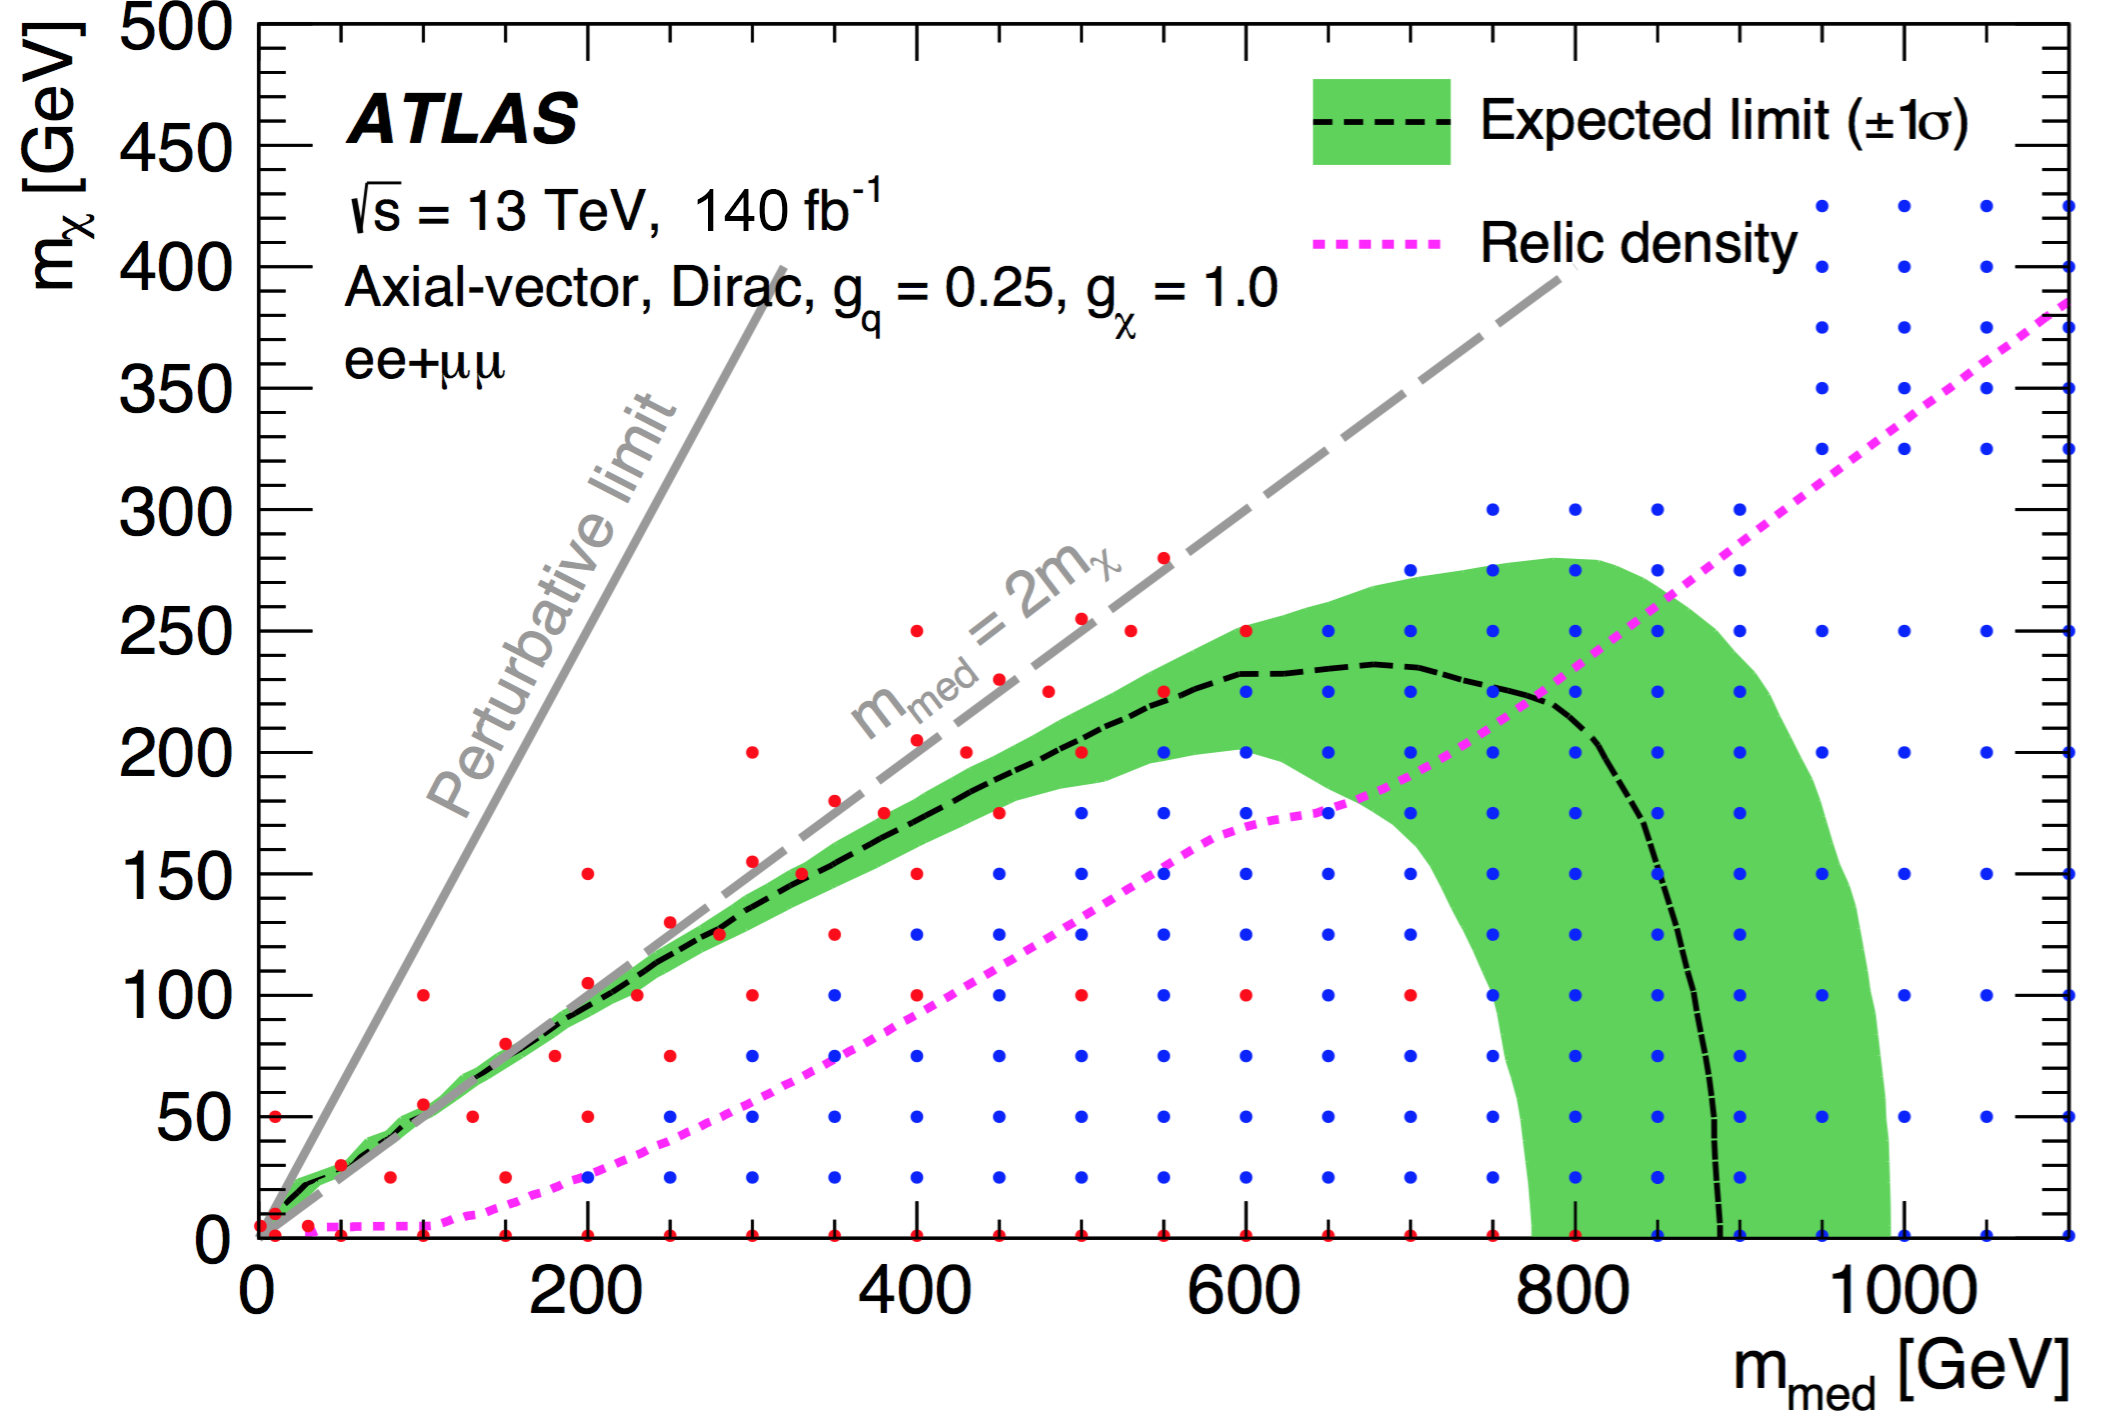
\includegraphics[width=0.7\textwidth]{Figures/140ifb.png}
\caption{Prospective vector exclusion limit with 140 \ifb. Produced by Chris Anelli.}
\label{fig:id}
\end{figure}

% --------------------------------------------------------------------------------------
\section{Other Analysis Improvements}

- comparison with ID measurements\\

\begin{figure}[htb]
\centering
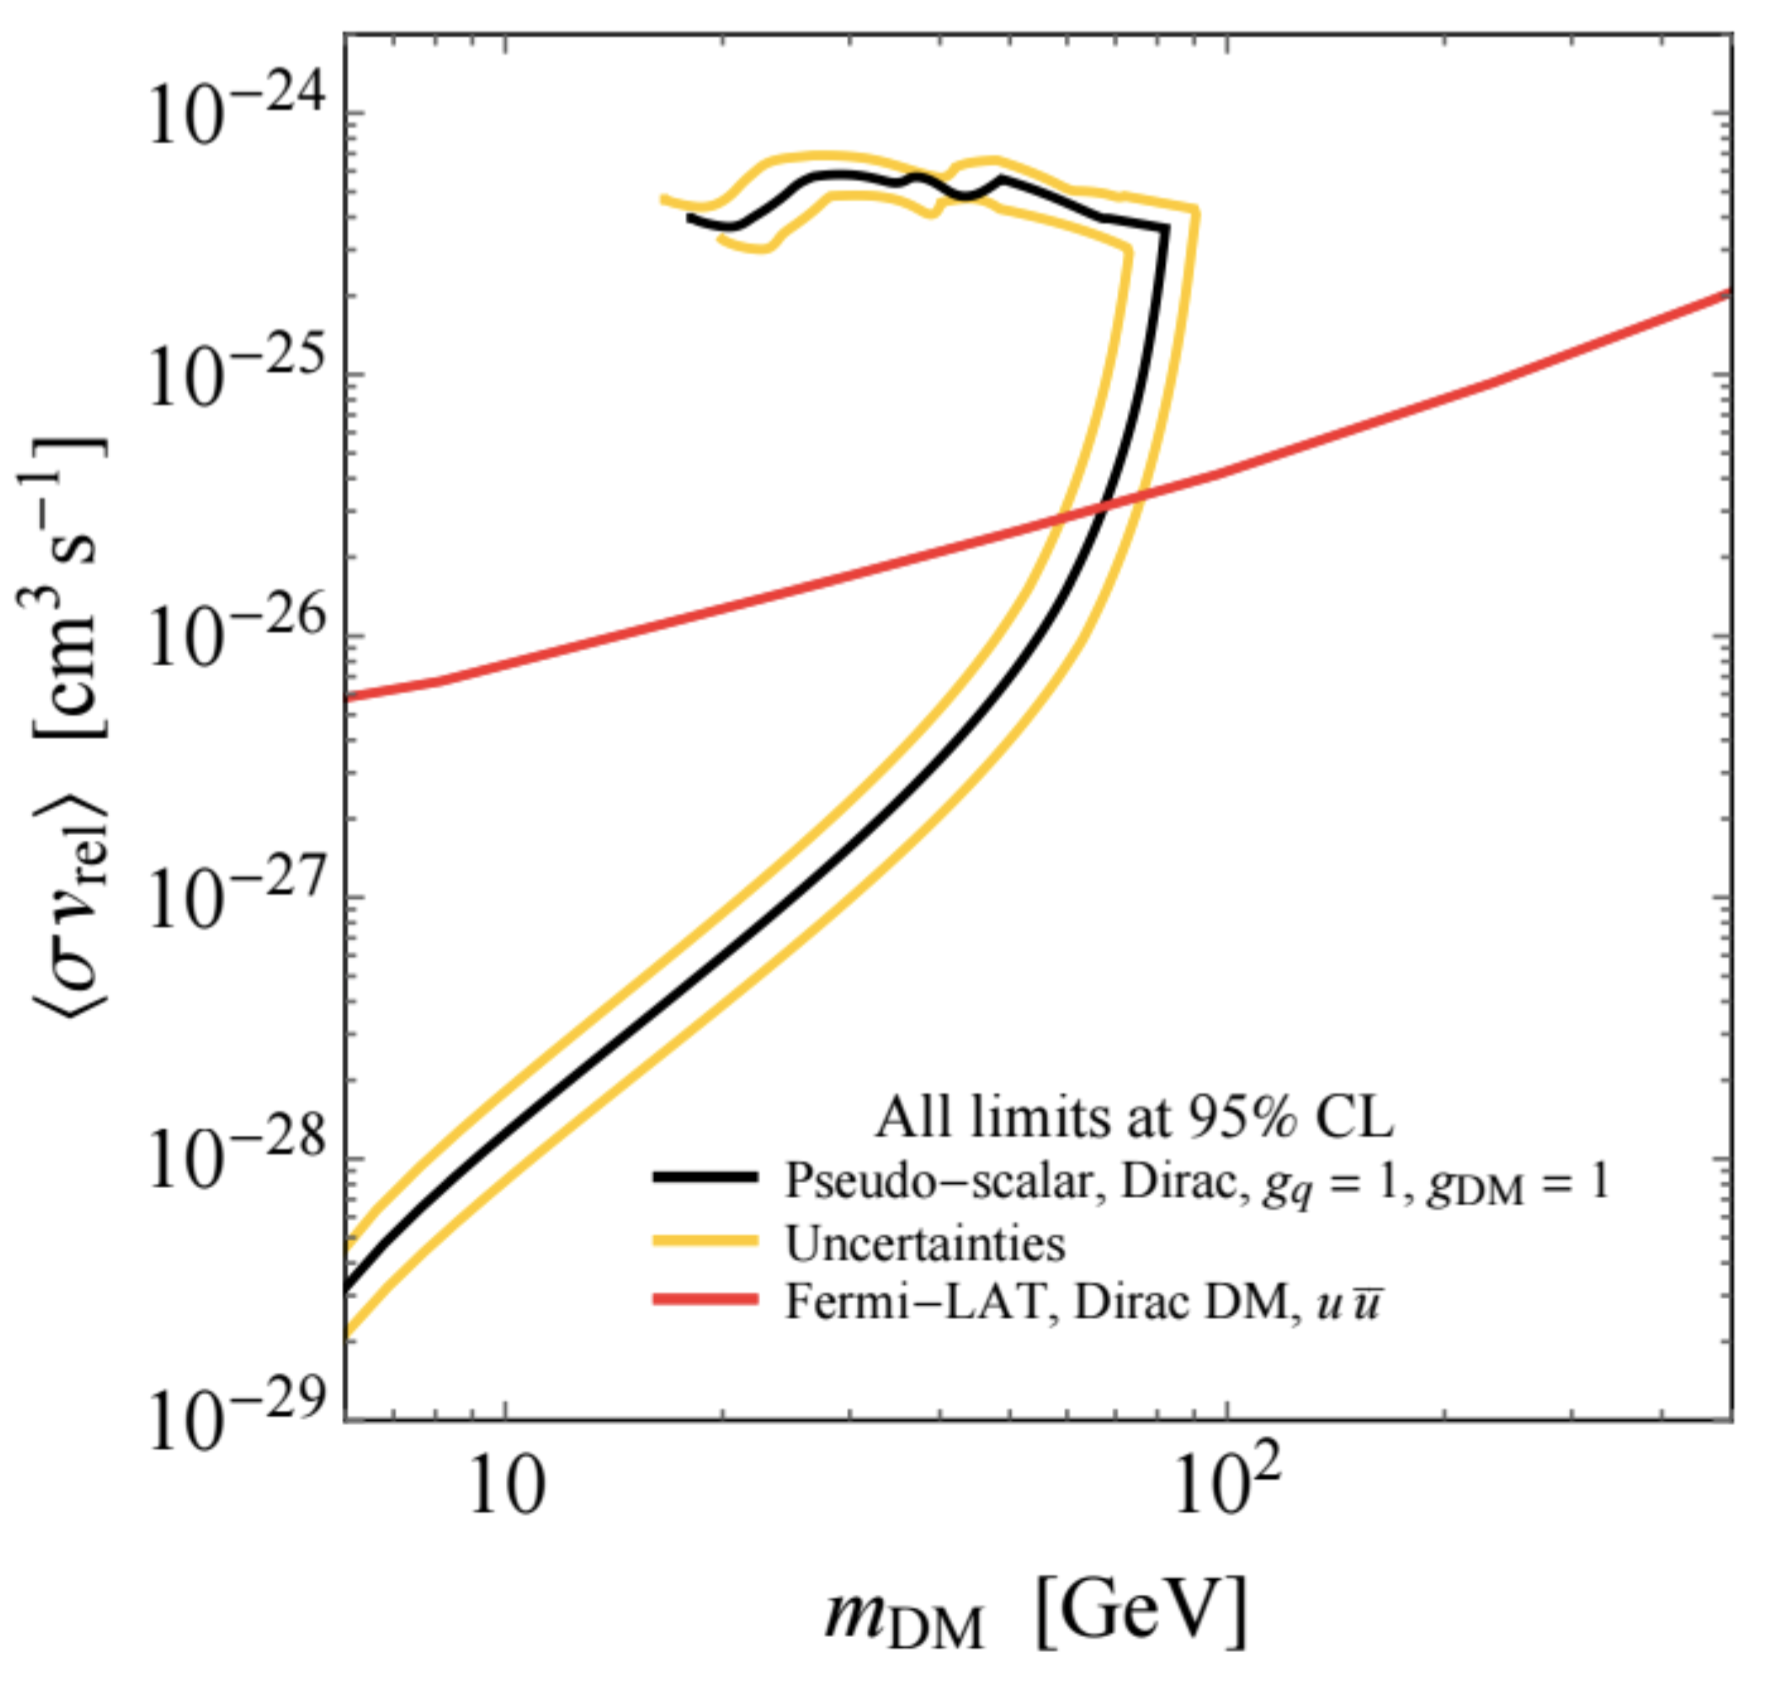
\includegraphics[width=0.5\textwidth]{Figures/id.png}
\caption{A schematic of what a comparison with ID detection measurements could look like.}
\label{fig:id}
\end{figure}

- theoretical uncertainties on signal acceptance - weights!! \\
- maintenance of analysis code\\